\documentclass{article}
\usepackage[utf8]{inputenc}
\usepackage{indentfirst}
\usepackage{titling}
\usepackage{geometry}
\usepackage{graphicx}
\usepackage{amsfonts}
\usepackage{mathtools}
\graphicspath{ {./img/} }
\usepackage[shortlabels]{enumitem}
\usepackage{fancyhdr}
\usepackage{ulem}
\usepackage[dvipsnames]{xcolor}
\usepackage{amsmath}


\renewcommand\maketitlehooka{\null\mbox{}\vfill} %para centralizar verticalmente
\renewcommand\maketitlehookd{\vfill\null}
\pagestyle{fancy}
\fancyhf{}
\rfoot{\thepage}
\lfoot{ 
\includegraphics[scale=0.01]{UA.jpg} José Mendes 107188 LEI}
\geometry{
  a4paper,
  headheight=4cm,
  top=5.5cm,
  bottom=4.5cm,
  footskip=4cm
}


\title{Compiladores - a partir do Cap. 5}
\author{José Mendes 107188}
\date{2023}

\begin{document}


\begin{titlepage}
    \maketitle
    \begin{center}
        
\includegraphics[scale=0.4]{UA.png}
    \end{center}
    \thispagestyle{empty} %remove o count da pagina
\end{titlepage}

\pagebreak
%depois por um index aqui

\section{Linguagens, Expressões e Gramáticas Regulares}

\subsection{Papel da análise lexical}

\begin{center}
  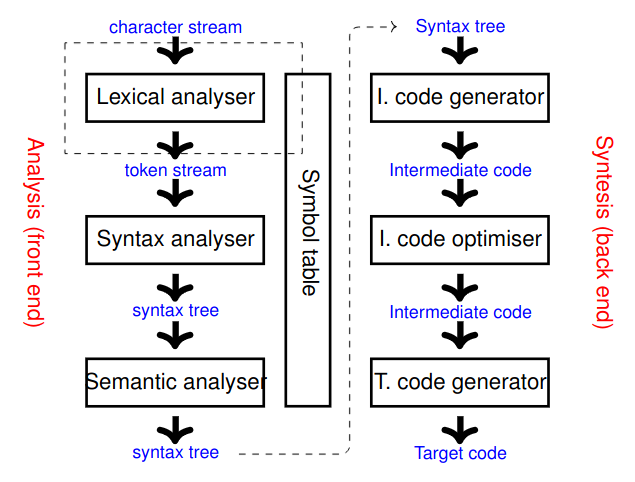
\includegraphics[scale=0.4]{1}
\end{center}

\begin{flushleft}
  \item Converte a sequência de caracteres numa sequência de \textbf{tokens}.
  \item Um \textbf{token} é um tuplo: $\textbf{$<$token-name, attrinute-value$>$}$.
  \begin{itemize}
    \item \uline{token-name} é um símbolo (abstrato), que representa um tipo de entrada;
    \item \uline{attribute-value} representa o valor corrente desse símbolo;
  \end{itemize}
  \item \textbf{Exemplo:}
  \[pos = pos + vel * 5\]
  é convertido em:
  \[<ID,"pos"> <=> <ID,"pos"> <+> <ID,"vel">
  <*> <INT,5>\]

  \item Tipicamente, alguns símbolos são descartados pelo analisador lexical.
  \item O conjunto dos tokens corresponde a uma linguagem regular
  \begin{itemize}
    \item os tokens são descritos usando expressões regulares e/ou gramáticas regulares;
    \item são reconhecidos usando autómatos finitos;
  \end{itemize}
\end{flushleft}

\pagebreak

\subsection{Linguagem Regular}

A classe das \textbf{linguagens regulares} sobre o alfabeto A define-se
indutivamente da seguinte forma:
\begin{itemize}
  \item O conjunto vazio, $\emptyset$, é uma linguagem regular (LR).
  \item Qualquer que seja o $a \in A$, o conjunto $\{a\}$  é uma LR.
  \vspace{-6mm}
  \begin{flushleft}
    \item \textbf{Nota:}
    \begin{itemize}
      \item em $a \in A$, $a$ é uma letra do alfabeto
      \item em $\{a\}$, $a$ é uma palavra com apenas uma letra
      \item Numa analogia Java, o primeiro é um 'a' e o segundo um "a"
    \end{itemize}
  \end{flushleft}

\item Se $L_1$ e $L_2$ são LR, então a sua reunião ($L_1 \cup L_2$) é uma LR.
\vspace{-6mm}
\begin{flushleft}
  \item \textbf{Exemplo:}
  \begin{itemize}
    \item Seja $L_1 = \{ab,c\}$, uma LR sobre o alfabeto $A = \{a,b,c\}$
    \item e $L_2 = \{bb,c\}$, outra LR sobre o mesmo alfabeto $A$
    \item então, $L_3 = L_1 \cup L_2 = \{ab,bb,c\}$ é uma LR sobre o mesmo alfabeto $A$
  \end{itemize}
\end{flushleft}

\item Se $L_1$ e $L_2$ são LR, então a sua concatenação $(L_1 \cdot L_2)$ é uma LR.
\vspace{-6mm}
\begin{flushleft}
  \item \textbf{Exemplo:}
  \begin{itemize}
    \item Seja $L_1 = \{ab,c\}$, uma LR sobre o alfabeto $A = \{a,b,c\}$
    \item e $L_2 = \{bb,c\}$, outra LR sobre o mesmo alfabeto $A$
    \item então, $L_3 = L_1 \cdot L_2 = \{abbb,abc, cbb, cc\}$ é uma LR sobre o mesmo alfabeto $A$
  \end{itemize}
\end{flushleft}

\item Se $L_1$ é uma LR, então o seu fecho de Kleene $(L_1)^*$ é uma LR.
\vspace{-6mm}
\begin{flushleft}
  \item \textbf{Exemplo:}
  \begin{itemize}
    \item Seja $L_1 = \{ab,c\}$, uma LR sobre o alfabeto $A = \{a,b,c\}$
    \item então, $L_2 = L_1^* = \{\varepsilon, ab, c, abab, abc, cab, cc, \dots\}$ é uma LR sobre o mesmo alfabeto $A$
  \end{itemize}
\end{flushleft}

\item Nada mais é LR.
\vspace{-6mm}
\begin{flushleft}
  \item \textbf{Nota:}
  \begin{itemize}
    \item $\{\varepsilon\}$ é uma LR, uma vez que $\{\varepsilon\} = \emptyset$
  \end{itemize}
\end{flushleft}
\end{itemize}

\pagebreak

\subsection{Definição de linguagem regular}

  \begin{center}
    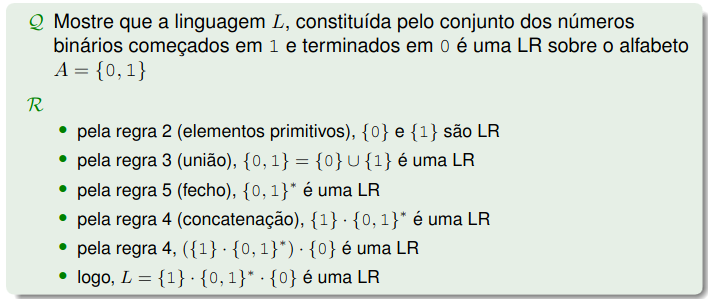
\includegraphics[scale=0.4]{27}
  \end{center}

\subsection{Expressões regulares}

\begin{flushleft}
  O conjunto das \textbf{expressões regulares} sobre o alfabeto A define-se
  indutivamente da seguinte forma:
  \begin{itemize}
    \item $\emptyset$ é uma expressão regular (ER) que representa LR $\{\}$.
    \item Qualquer que seja o $\alpha \in A$, $\alpha$ é uma ER que representa a LR $\{\alpha\}$
    \item Se $e_1$ e $e_2$ são ER representando respetivamente as LR $L_1$ e $L_2$, então $(e_1 | e_2)$ é uma
    ER representando a LR $L_1 \cup L_2$.
    \item Se $e_1$ e $e_2$ são ER representando respetivamente as LR $L_1$ e $L_2$, então $(e_1  e_2)$ é uma
    ER representando a LR $L_1 \cdot L_2$.
    \item  Se $e_1$ é uma ER representando a LR $L_1$, então $(e_1)^*$ é uma ER representando a LR $(L_1)^*$
    \item Nada mais é uma expressão regular.
  \end{itemize}

  \textbf{Nota:} É habitual representar-se por $\varepsilon$ a ER $\emptyset^*$. Representa a linguagem $\{\varepsilon\}$

  \item Na escrita de expressões regulares assume-se a seguinte precedência
  dos operadores:
  \begin{itemize}
    \item fecho (*)
    \item concatenação
    \item escolha ($|$)
  \end{itemize}

  \item O uso destas precedências permite a queda de alguns parêntesis e consequentemente uma
  notação simplificada.

  \item \textbf{Exemplo:} $e_1 | e_2 e_3^*$ recorre a precedência para representar a expressão regular: $(e_1) | (e_2((e_3)^*))$
\end{flushleft}

\pagebreak

\begin{flushleft}
  \textbf{Exemplos:}

  \begin{center}
    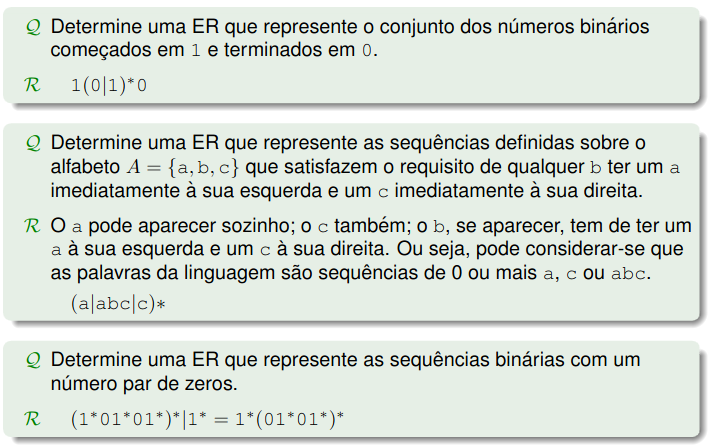
\includegraphics[scale=0.4]{2}
  \end{center}

  \item A operação de escolha goza das propriedades:
  \begin{itemize}
    \item comutativa: $e_1 | e_2 = e_2 | e_1$
    \item associativa: $e_1 | (e_2 | e_3) = (e_1 | e_2) | e_3 = e_1 | e_2 | e_3$
    \item idempotência: $e_1 | e_1 = e_1$
    \item existência de elemento neutro: $e_1 | \emptyset = \emptyset | e_1 = e_1$ 
  \end{itemize}

  \item A operação de concatenação goza das propriedades:
  \begin{itemize}
    \item associativa: $e_1  (e_2  e_3) = (e_1  e_2)  e_3 = e_1  e_2  e_3$
    \item existência de elemento neutro: $e_1  \varepsilon = \varepsilon  e_1 = e_1$ 
    \item existência de elemento absorvente $e_1 \emptyset = \emptyset e_1 = \emptyset$
    \item \textbf{não goza da propriedade comutativa}
  \end{itemize}

  \item A combinação das operações de concatenação e escolha gozam das propriedades:
  \begin{itemize}
    \item distributiva à esquerda da concatenação em relação à escolha:
    \[e_1 | (e_2 | e_3) = e_1 e_2 | e_1 e_3\]
    \item distributiva à direita da concatenação em relação à escolha:
    \[(e_1 | e_2) e_3 = e_1 e_3 | e_2 e_3\]
  \end{itemize}

  \pagebreak

  \item A operação de fecho goza das propriedades:
  \begin{itemize}
    \item $(e^*)^* = e^*$
    \item $(e_1^* | e_2^*)^* = (e_1 | e_2)^*$
    \item $(e_1 | e_2^*)^* = (e_1 | e_2)^*$
    \item $(e_1^* | e_2)^* = (e_1 | e_2)^*$
  \end{itemize}
  \item Mas \textbf{atenção}:
  \begin{itemize}
    \item $(e_1 | e_2)^* \ne e_1^* | e_2^*$
    \item $(e_1  e_2)^* \ne e_1^*  e_2^*$
  \end{itemize}

  \textbf{Exemplos:}

  \begin{center}
    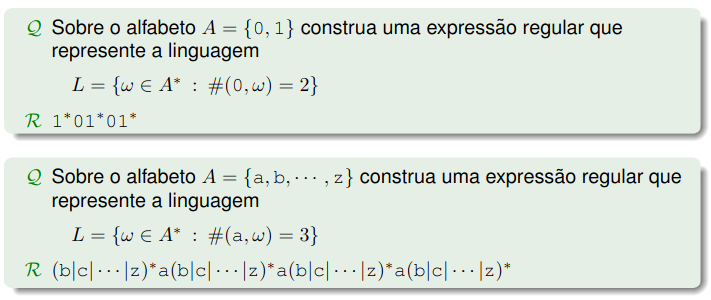
\includegraphics[scale=0.4]{3}
  \end{center}
    Na  última resposta, onde estão as reticências (\dots) deveriam estar todas as letras
  entre d e y. Parece claro que faz falta uma forma de simplificar este tipo de
  expressões
\end{flushleft}


\subsubsection{Extensões notacionais comuns}

\begin{flushleft}
    \item $\rightarrow$ Uma ou mais ocorrências: $e^+ = e \cdot e^*$
    \item $\rightarrow$ Uma ou nenhuma ocorrência: $e? = (e | \varepsilon)$
    \item $\rightarrow$ Um símbolo do sub-alfabeto dado: $[a_1a_2a_3 \dots a_n] = (a_1|a_2|a_3|\dots|a_n)$
    \item $\rightarrow$ Um símbolo do sub-alfabeto dado: $[a_1 - a_n] = (a_1 | \dots | a_n)$
    \item $\rightarrow$ Um símbolo do alfabeto fora do conjunto dado: $[\hspace{1mm}\hat{}\hspace{1mm} a_1a_2a_3 \dots a_n]$, $[\hspace{1mm}\hat{}\hspace{1mm} a_1 - a_n]$
    \item $\rightarrow$ n ocorrência de: $ e\{n\} = \underbrace{e . e . \dots . e}_n$
    \item $\rightarrow$ de $n_1$ a $n_2$ ocorrências: $e\{n_1,n_2\} = \underbrace{e . e . \dots . e}_{n_1, n_2}$
    \item $\rightarrow$ n ou mais ocorrências: $e\{n,\} = \underbrace{e . e . \dots . e}_{n,}$
    \item $\rightarrow$ "$.$" representa um símbolo Qualquer
    \item $\rightarrow$ "$\hat{}$" representa palavra vazia no início de linha
    \item $\rightarrow$ "\$" representa palavra vazia no fim de linha
    \item $\rightarrow$ "$\backslash <$" representa palavra vazia no ínicio de palavra
    \item $\rightarrow$ "$\backslash >$" representa palavra vazia no fim de palavra
    \break

    \textbf{Exemplo:}

    \begin{center}
      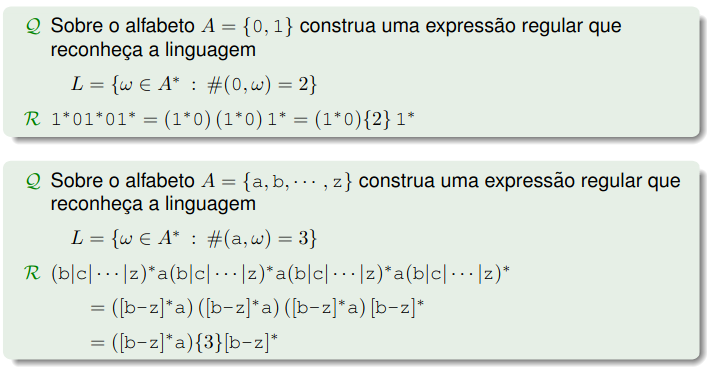
\includegraphics[scale=0.4]{4}
    \end{center}

\end{flushleft}


\subsection{Gramáticas regulares}

\begin{flushleft}
  \textbf{Exemplo de gramática regular:}

  \begin{align*}
      S & \rightarrow a\hspace{1mm} X \\
      X & \rightarrow a\hspace{1mm} X \\
      & | \hspace{1mm}b\hspace{1mm} X \\
      & | \hspace{1mm} \varepsilon
  \end{align*}
\end{flushleft}

\begin{flushleft}
  \textbf{Exemplo de gramática \uline{não} regular:}

  \begin{align*}
      S & \rightarrow a\hspace{1mm} S\hspace{1mm} a\\
      X & \rightarrow b\hspace{1mm} S\hspace{1mm} b \\
      & | \hspace{1mm} a \\
  \end{align*}

  \item Letras minúsculas representam símbolos terminais e letras maísculas
  representam símbolos não terminais (o contrário do ANTLR).

  \item Nas gramáticas regulares os símbolos não terminais apenas podem aparecer no
  fim.
\end{flushleft}

\pagebreak

\begin{flushleft}
  \item Uma \textbf{gramática regular} é um quádruplo $G = (T, N, P, S)$ onde:
  \begin{itemize}
    \item $T$ é um conjunto finito não vazio de símbolos terminais;
    \item $N$, sendo $N \cap T = \emptyset$, é um conjunto finito não vazio de símbolos não terminais;
    \item $P$ é um conjunto de produções (ou regra de rescrita), cada uma da forma $\alpha \rightarrow \beta$, onde;
    \begin{itemize}
      \item $\alpha \in N$
      \item $\beta \in T^* \cup T^* N$
    \end{itemize}
    \item $S \in N$ é o símbolo inicial.
  \end{itemize}

  \begin{itemize}
    \item A linguagem gerada por uma gramática regular  é regular.
    
    Logo, é possível converter-se uma gramática regular numa expressão regular que
    represente a mesma linguagem e vice-versa.
  \end{itemize}
\end{flushleft}

\subsubsection{Operações sobre gramáticas regulares}

\begin{flushleft}
  \item As gramáticas regulares são fechadas sob as operações de:
  \begin{itemize}
    \item reunião
    \item concatenação
    \item fecho
    \item interseção
    \item complementação
  \end{itemize}

  \item As operações de interseção e complementação serão abordadas mais adiante através
  de autómatos finitos 

  \pagebreak

  \subsubsection{Reunião de gramáticas regulares}

  \item \textbf{Exemplo:}

  \begin{center}
    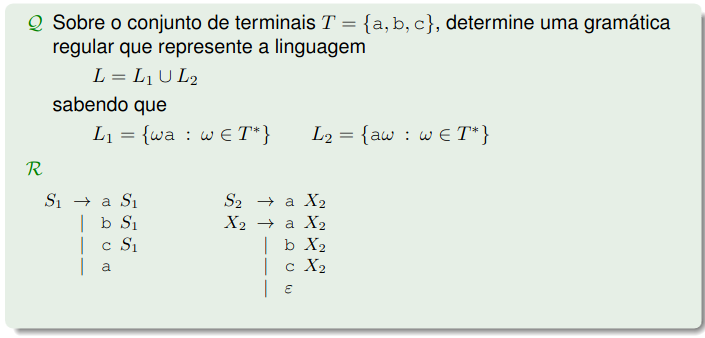
\includegraphics[scale=0.4]{5}
  \end{center}

  Comece-se por obter as gramáticas regulares que representam $L_1$ e $L_2$.

  \begin{center}
    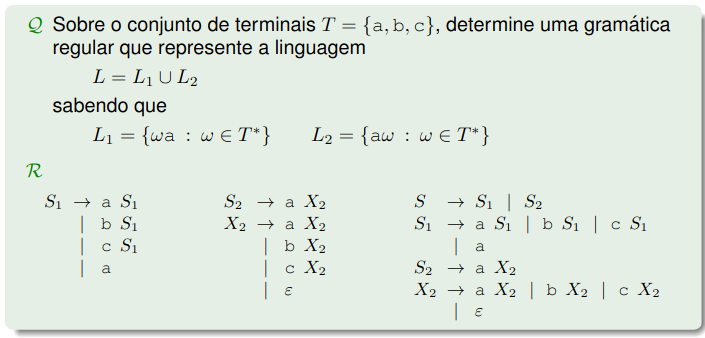
\includegraphics[scale=0.4]{6}
  \end{center}
  
  E acrescenta-se as transições $S \rightarrow S_1$ $S \rightarrow S_2$ que permitem
  escolher as palavras de $L_1$ e de $L_2$, sendo $S$ o novo símbolo inicial.   

  \item \textbf{Algoritmo:}

  \begin{center}
    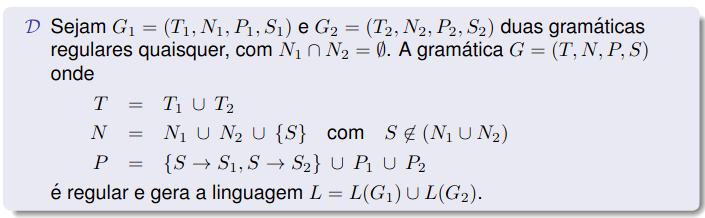
\includegraphics[scale=0.4]{7}
  \end{center}

  \item Para $i = 1,2,$ a nova produção $S \rightarrow S_i$ permite que $G$ gere a linguagem $L(G_i)$
\end{flushleft}


\pagebreak

\subsubsection{Concatenação de gramáticas regulares}

\begin{flushleft}
  \textbf{Exemplo:}

  \begin{center}
    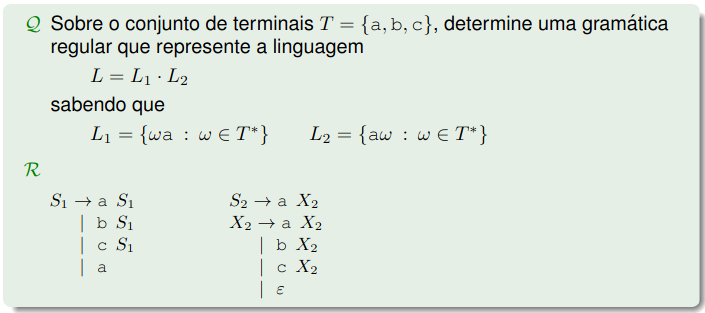
\includegraphics[scale=0.4]{8}
  \end{center}

  Comece-se por obter que representam $L_1$ e $L_2$.

  \begin{center}
    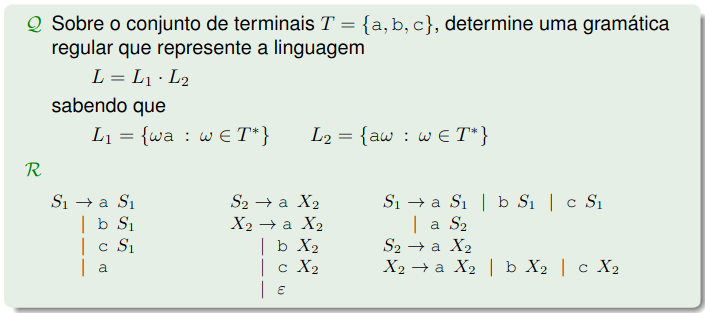
\includegraphics[scale=0.4]{9}
  \end{center}

  A seguir substitui-se $S_1 \rightarrow a$ por $S_1 \rightarrow a \hspace{1mm} S_2$,
  de modo a impor que a segunda parte das palavras têm de pertemcer a $L_2$.

  \item \textbf{Algoritmo:}
  
  \begin{center}
    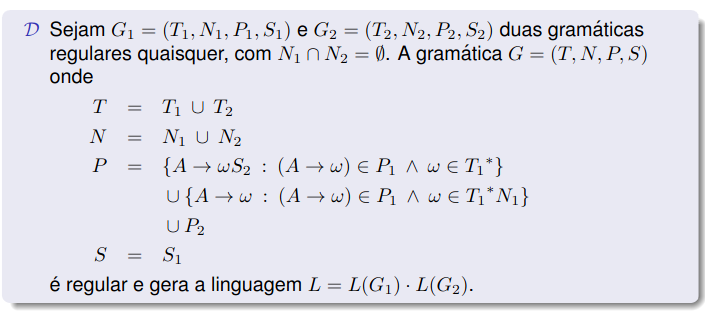
\includegraphics[scale=0.4]{10}
  \end{center}

  \item As produções da primeira gramática do tipo $\beta \in T^*$ ganham o símbolo
  inicial da segunda gramática no fim.
  \item As produções da primeira gramática do tipo $\beta \in T^* N$ mantêm-se inalteradas.
  \item As produções da segunda gramática mantêm-se inalteradas.

\end{flushleft}

\subsubsection{Fecho de gramáticas regulares}

\begin{flushleft}
  \begin{center}
    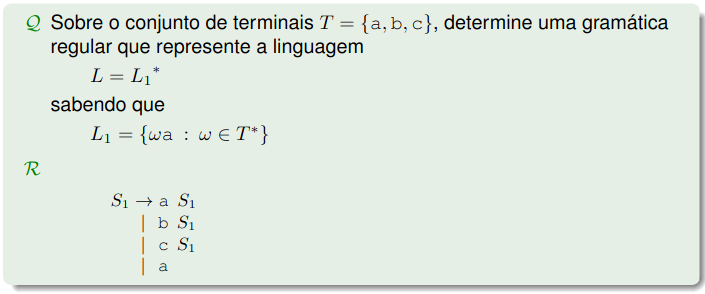
\includegraphics[scale=0.4]{11}
  \end{center}

  Começa-se pela obtenção da gramática regular que representa $L_1$.

  \begin{center}
    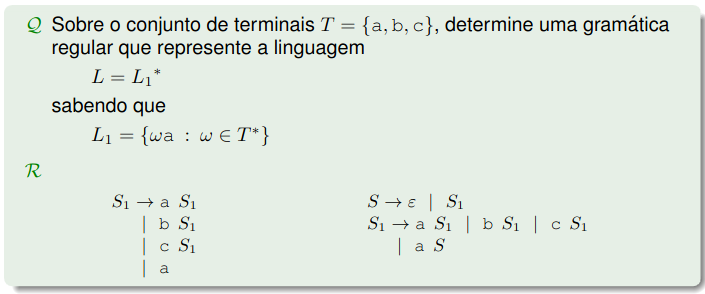
\includegraphics[scale=0.4]{12}
  \end{center}

  \item Acrescentando-se a transição $S \rightarrow S_1$ e substituindo-se $S_1 \rightarrow a$
  por $S_1 \rightarrow a \hspace{1mm} S$, permite-se iterações sobre $S_1$.
  \item Acrescentando-se $S \rightarrow \varepsilon$, permite-se 0 ou mais iterações.

  \item \textbf{Algoritmo:}
  
  \begin{center}
    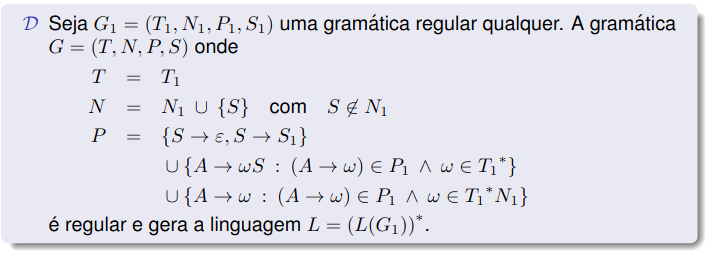
\includegraphics[scale=0.4]{13}
  \end{center}

  \item As novas produções $S \rightarrow \varepsilon$ e $S \rightarrow S_1$ garantem que
  $(L(G_1))^* \subseteq L(G)$, para qualquer $n \ge 0$.
  \item As produções que só têm terminais ganham o novo símbolo inicial no fim.
  \item As produções que terminam num não terminal mantêm-se inalteradas.
\end{flushleft}

\pagebreak

\subsection{Conversão de uma ER em um GR}

\begin{flushleft}
  \subsubsection{Exemplo}

  \begin{center}
    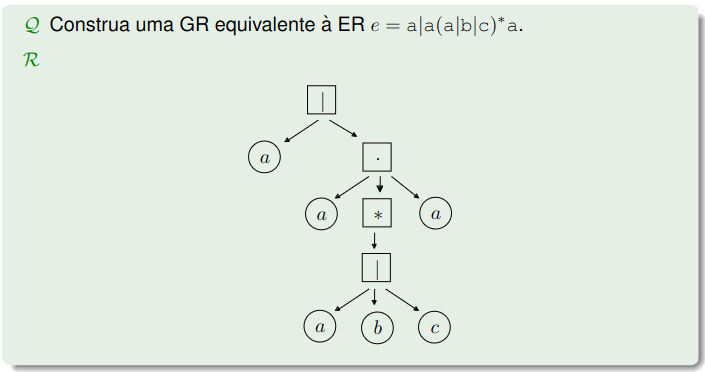
\includegraphics[scale=0.4]{14}
  \end{center}
  \item Coloque-se de forma arbórea.

  \begin{center}
    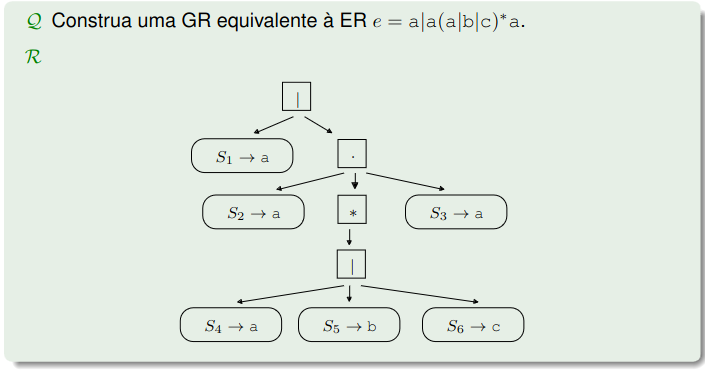
\includegraphics[scale=0.4]{15}
  \end{center}
  \item Após converter as folhas (elementos primitivos) em GR.

  \begin{center}
    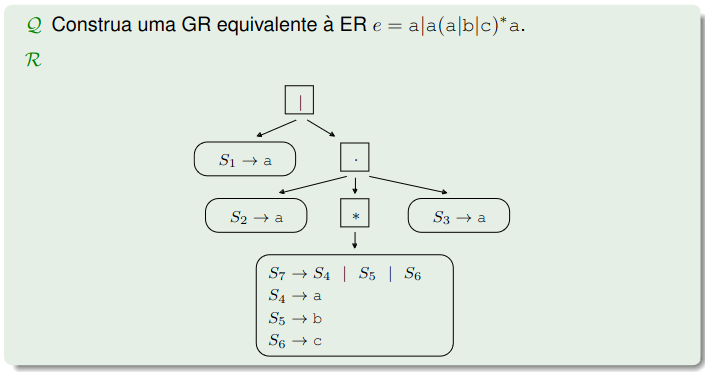
\includegraphics[scale=0.4]{16}
  \end{center}
  \item Após aplicar a escolha (reunião) de baixo.

  \pagebreak

  \begin{center}
    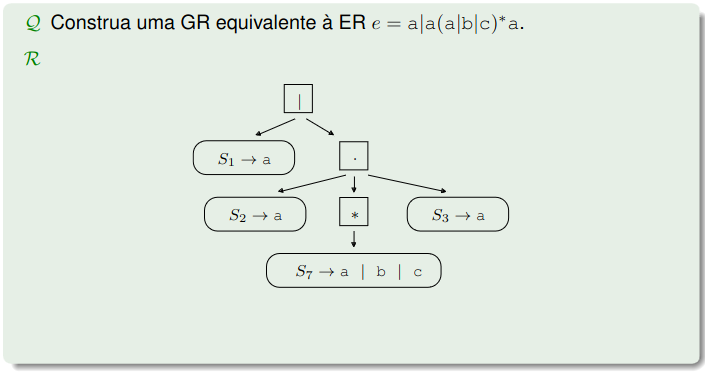
\includegraphics[scale=0.4]{17}
  \end{center}
  \item Simplificando.
  
  \begin{center}
    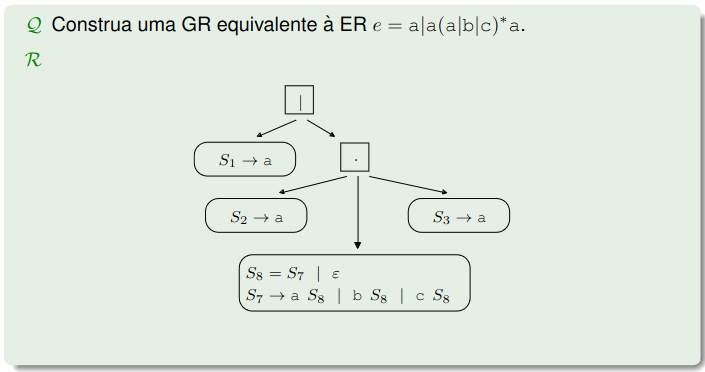
\includegraphics[scale=0.4]{18}
  \end{center}
  \item Após aplicar o fecho.

  \begin{center}
    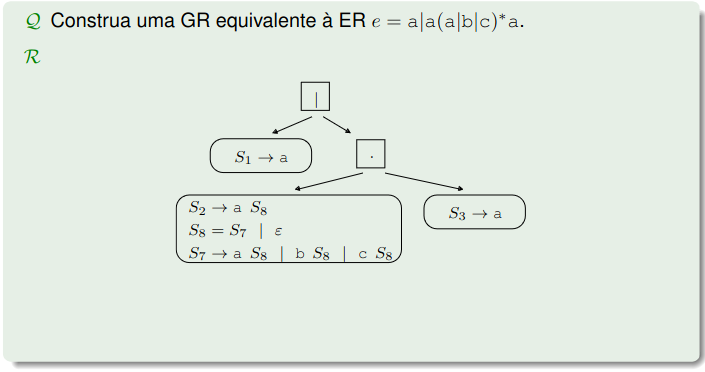
\includegraphics[scale=0.4]{19}
  \end{center}
  \item Após aplicar a concatenação.

  \begin{center}
    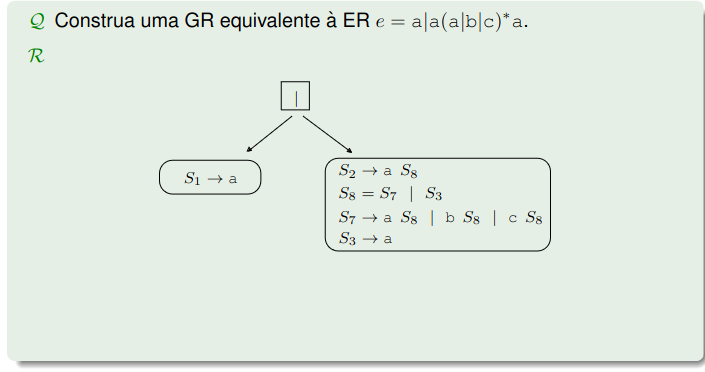
\includegraphics[scale=0.4]{20}
  \end{center}
  \item Após aplicar a concatenação da direita.


  \begin{center}
    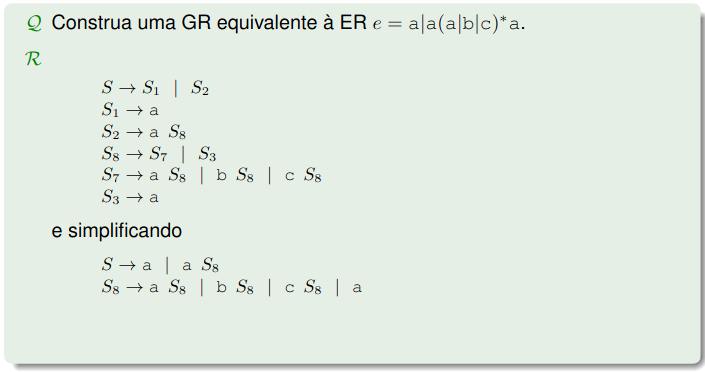
\includegraphics[scale=0.4]{21}
  \end{center}
  \item Finalmente após aplicar escolha (reunião) de cima.

  \subsubsection{Abordagem}

  \item Dada uma expressão regular qualquer ela é:
  \begin{itemize}
    \item ou um elemento primitivo;
    \item ou uma expressão do tipo $e^*$, sendo $e$ uma expressão regular qualquer;
    \item ou uma expressão do tipo $e_1 \cdot e_2$, sendo $e_1$ e $e_2$ duas expressões regulares quaisquer;
    \item ou uma expressão do tipo $e_1 \hspace{1mm} | \hspace{1mm}$, sendo $e_1$ e $e_2$ duas expressões regulares quaisquer.
  \end{itemize}

  \item Identificando-se as GR equivalentes às ER primitivas, tem-se o problema resolvido, visto
  que se sabe como fazer a reunião, a concatenação e o fecho de GR.

  \begin{center}
    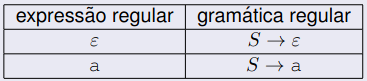
\includegraphics[scale=0.4]{22}
  \end{center}

  \pagebreak

  \subsubsection{Algoritmo de conversão}

  \begin{enumerate}
    \item Se ER é do tipo primitivo, a GR correspondente pode ser obtido da tabela anterior.
    \item Se é do tipo $e^*$, aplica-se este mesmo algoritmo na obtenção de uma GR equivalente
    à expressão regular $e$ e, de seguida,, aplica-se o fecho de GR.
    \item Se é do tipo $e_1 \cdot e_2$, aplica-se este mesmo algoritmo na obtenção de uma GR para
    as expressões $e_1$ e $e_2$, de seguida, aplica-se a concatenação de GR.
    \item Finalmente, se é do tipo $e_1 \hspace{1mm} | \hspace{1mm} e_2$, aplica-se este mesmo algoritmo na
    obtenção de GR para as expressões $e_1$ e $e_2$, de seguida, aplica-se a reunião de GR.
  \end{enumerate}

  \item (Na realidade, o algoritmo corresponde a um processo de decomposição arbórea a partir
  da raiz seguido de um processo de construção arbórea a partir das folhas).

  \subsection{Conversão de uma GR em uma ER}

  \subsubsection{Exemplo}

  \begin{center}
    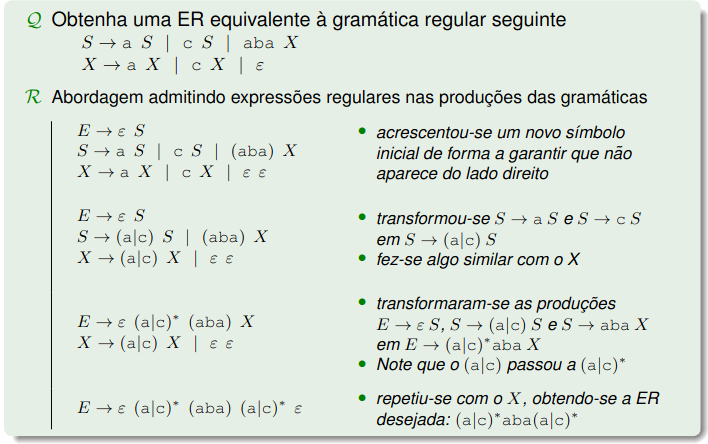
\includegraphics[scale=0.399]{23}
  \end{center}

  \begin{center}
    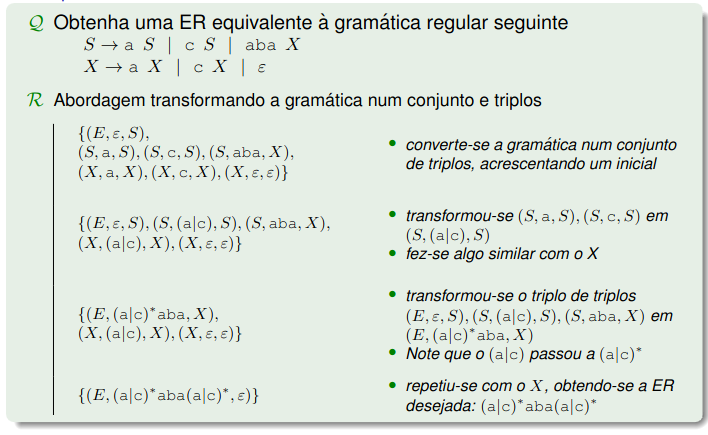
\includegraphics[scale=0.399]{24}
  \end{center}

  \pagebreak

  \subsubsection{Algoritmo}

  \begin{center}
    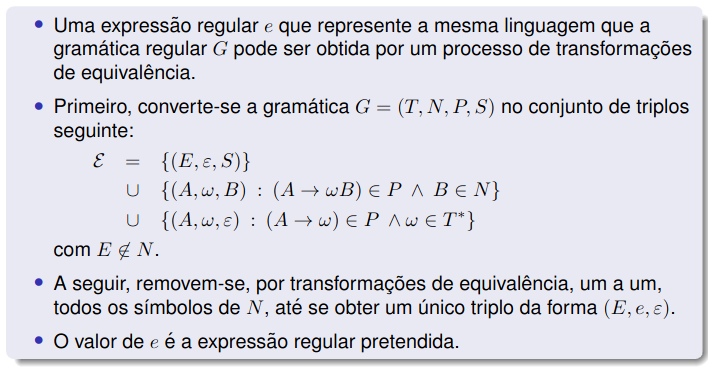
\includegraphics[scale=0.4]{25}
  \end{center}

  \begin{center}
    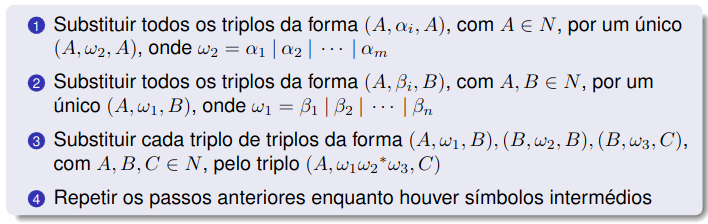
\includegraphics[scale=0.4]{26}
  \end{center}

  \item Note que, se não existir qualquer triplo do tipo $(A, \alpha_i, A)$, $w_2$ representa
  o consjunto vazio e consequentemente $w_2^* = \varepsilon$
\end{flushleft}

\section{Atómatos Finitos}

\begin{flushleft}
  \textbf{Autómato Finito -} é um mecanismo reonhecedor das palavras de uma linguagem regular.
  \vspace{4mm}
  \begin{center}
    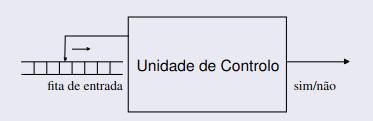
\includegraphics[scale=0.5]{28}
  \end{center}
  \item A unidade de controlo é baseada nas noções de estado e de transição entre estados (número finito de estados).
  \item A fita de entrada é só de leitura, com acesso sequencial.
  \item Os autómatos finitos podem ser \textbf{deterministas}, \textbf{não deterministas} ou \textbf{generalizados}.
\end{flushleft}

\break

\subsection{Autómato finito determinista}

\begin{flushleft}
  \begin{center}
    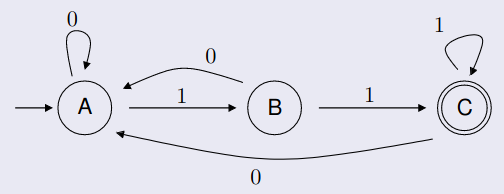
\includegraphics[scale=0.5]{29}
  \end{center}

  \item Um \textbf{autómato finito determinista} é um autómato finito onde:
  \begin{itemize}
    \item as transições estão associadas a símbolos individuais do alfabeto;
    \item de cada estado sai \textbf{uma e uma só} transição por cada símbolo do alfabeto;
    \item há um estado inicial;
    \item há 0 ou mais estados de aceitação, que determinam as palavras aceites;
    \item os caminhos que começam no estado inicial e terminam num estado de aceitação representam as
    palavras aceites (reconhecidas) pelo autómato.
  \end{itemize}

  \subsubsection{Exemplos}

  \begin{center}
      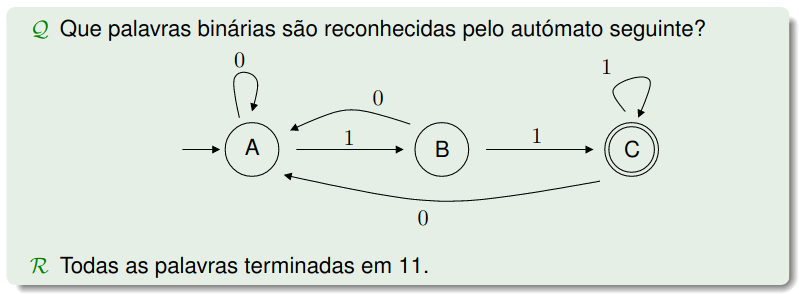
\includegraphics[scale=0.4]{30}
  \end{center}

    A expressão seria:
    \[(0 \hspace{1mm} | \hspace{1mm} 1)^* \hspace{1mm} 11\]

    \begin{center}
      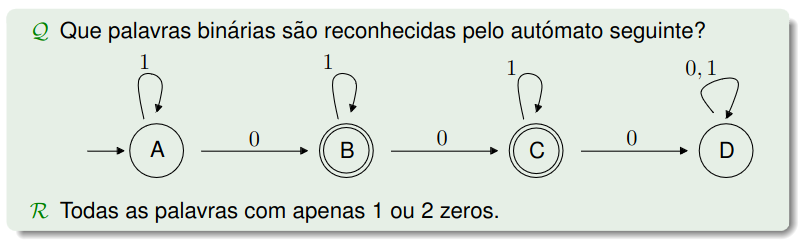
\includegraphics[scale=0.4]{31}
  \end{center}
  A expressão seria (acho eu):
    \[ 1^* \hspace{1mm} 0 \hspace{1mm} 1^* \hspace{1mm} 0 \hspace{1mm} 1^*\]

  \pagebreak

  \begin{center}
    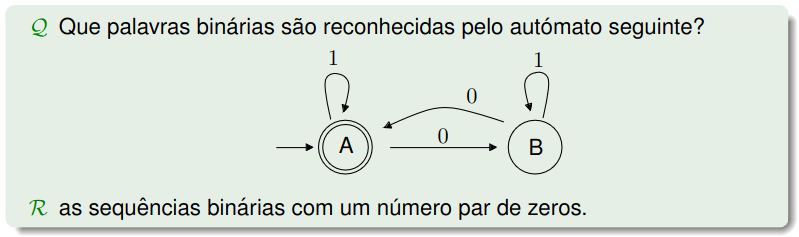
\includegraphics[scale=0.4]{32}
  \end{center}

A expressão seria (acho eu):
    \[ (1^* \hspace{1mm} 0 \hspace{1mm} 1^* \hspace{1mm} 0 \hspace{1mm} 1^*)^*\]
\end{flushleft}

\subsubsection{Definição de um autómato finito determinista}

\begin{flushleft}
  \item Um autómato finito determinista (AFD) é um quíntuplo $M = (A,Q,q_0, \delta, F)$, em que:
  \begin{itemize}
    \item $A$ é o alfabeto de entrada;
    \item $Q$ é um conjunto finito não vazio de estados;
    \item $q_0 \in Q$ é o estado inicial;
    \item $\delta : \hspace{1mm} Q \times A \rightarrow Q$ é uma função que determina a transição entre estados;
    \item $F \subseteq Q$ é o conjunto dos estados de aceitação.
  \end{itemize}
\end{flushleft}
\vspace{4mm}
\textbf{Exemplo:}\hfill

\begin{center}
  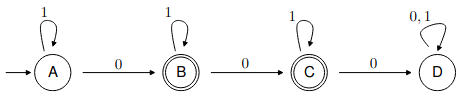
\includegraphics[scale=0.5]{33}
\end{center}

\begin{align*}
  & A = \{0,1\}\\
  & Q = \{A, B, C, D\}\\
  & q_0 = A\\
  & F \{B, C\}
\end{align*}


\begin{center}
  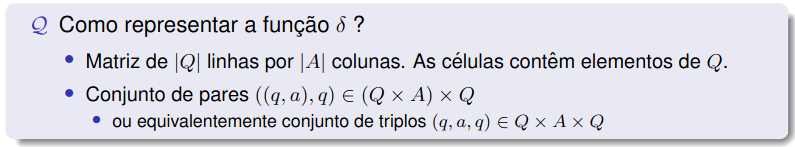
\includegraphics[scale=0.4]{34}
\end{center}

\pagebreak

\begin{center}
  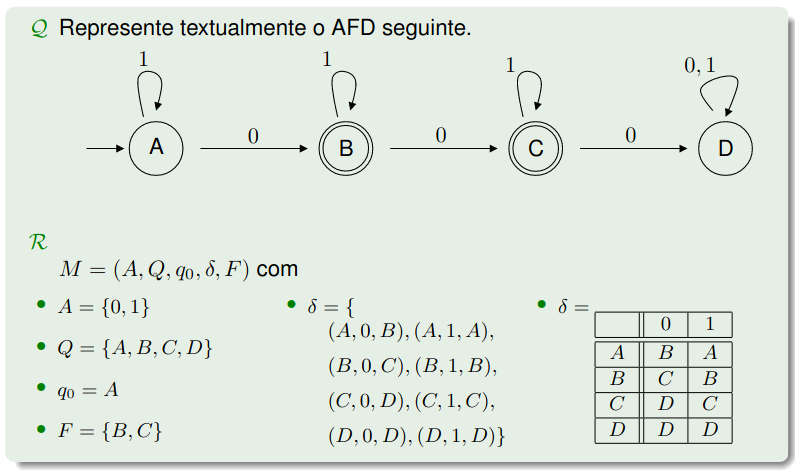
\includegraphics[scale=0.4]{35}
\end{center}

\subsubsection{Linguagem reconhecida por um AFD}

Diz-se que um AFD $M = (A, Q, q_0, \delta, F)$, \textbf{aceita} uma palavra $u \in A^*$
se $u$ se puder escrever na forma $u = u_1u_2 \dots u_n$ e existir uma sequência de estados
$s_0,s_1, \dots, s_n,$ que satisfaça as seguintes condições:
\begin{itemize}
  \item $s_0 = q_0^*$;
  \item qualquer que seja o $i = 1, \dots, n$, $s_i = \delta (s_{i-1}, u_i)$;
  \item $s_n \in F$.
\end{itemize} 
Caso contrário diz-se que $M$ \textbf{rejeita} a sequência de entrada.

\begin{center}
  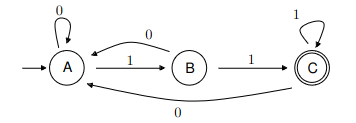
\includegraphics[scale=0.5]{36}
\end{center}

\begin{center}
  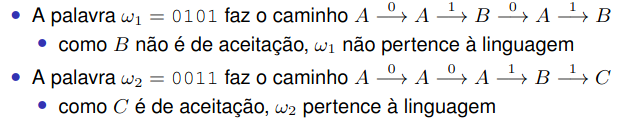
\includegraphics[scale=0.5]{37}
\end{center}

\pagebreak

\begin{center}
  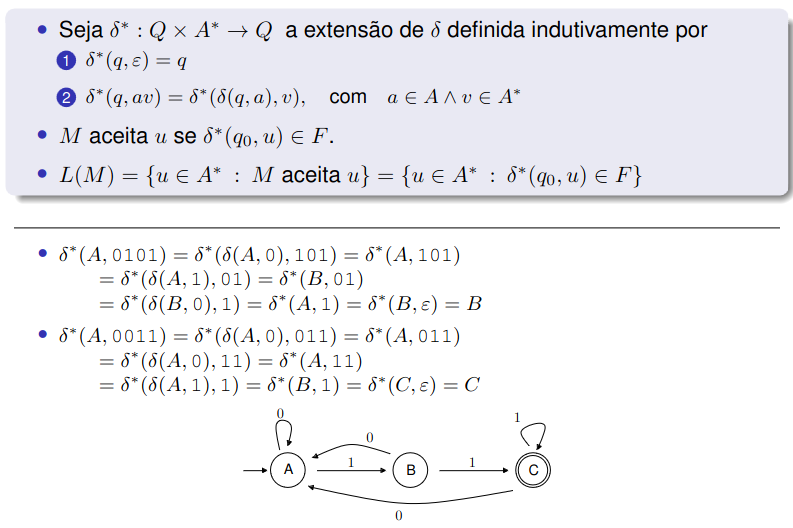
\includegraphics[scale=0.5]{38}
\end{center}

\subsubsection{Linguagem para Autómato}

\begin{center}
  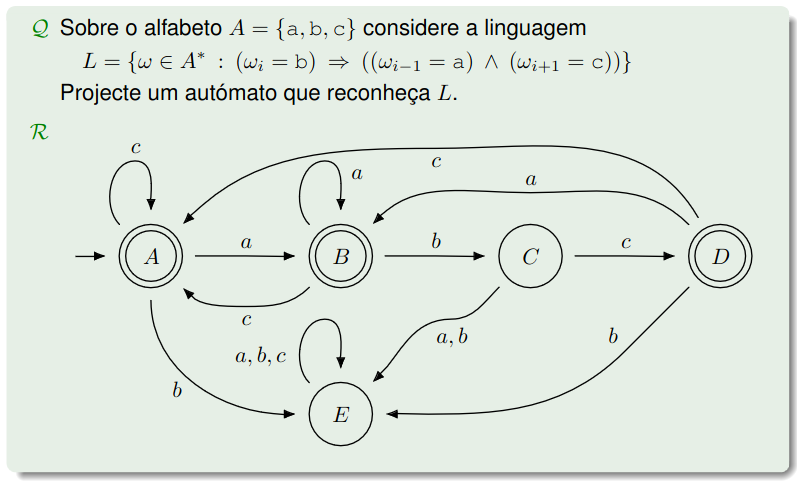
\includegraphics[scale=0.4]{39}
  \break
  \textcolor{BrickRed}{** Este aqui **}
\end{center}

\begin{center}
  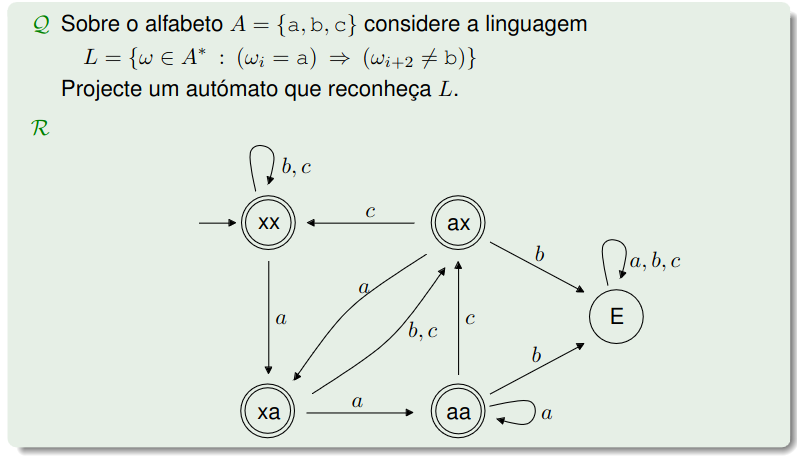
\includegraphics[scale=0.4]{40}
\end{center}
\hfill

\subsubsection{Redução de um AFD}

\begin{flushleft}
  No exemplo a duas imagens a cima, comparando os estados $A$ e $C$ concluímos que
  as suas transições são iguais (para os mesmos estados), podemos dizer que são \textbf{equivalentes}.
  Por consequente podem ser fundidos.

  \begin{center}
    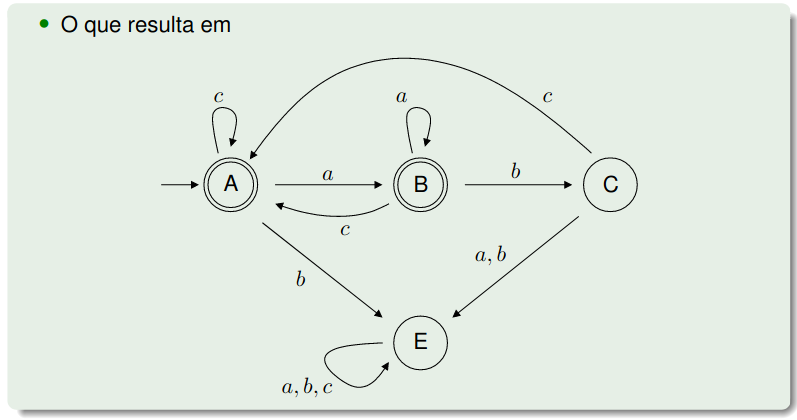
\includegraphics[scale=0.4]{41}
  \end{center}

  Este pode provar-se, no tem estados redundantes. Está no estado \textbf{reduzido}.
\end{flushleft}

\subsubsection{Algoritmo de redução de AFD}

\begin{flushleft}
  \begin{center}
    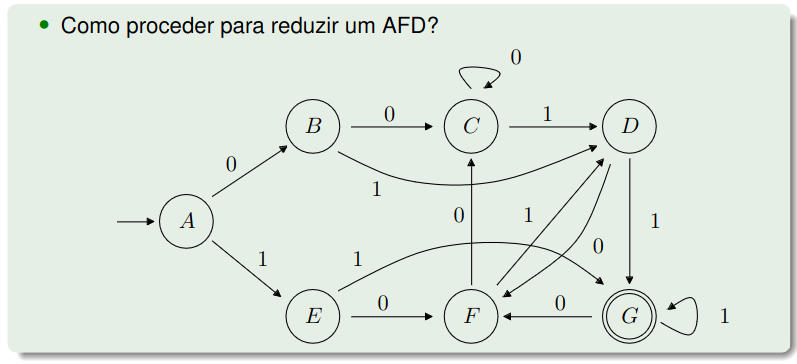
\includegraphics[scale=0.4]{42}
  \end{center}

  \item Primeiro, divide-se os estados em dois conjuntos, um contendo os estados
  de aceitação e outro os de não-aceitação.

  \begin{center}
    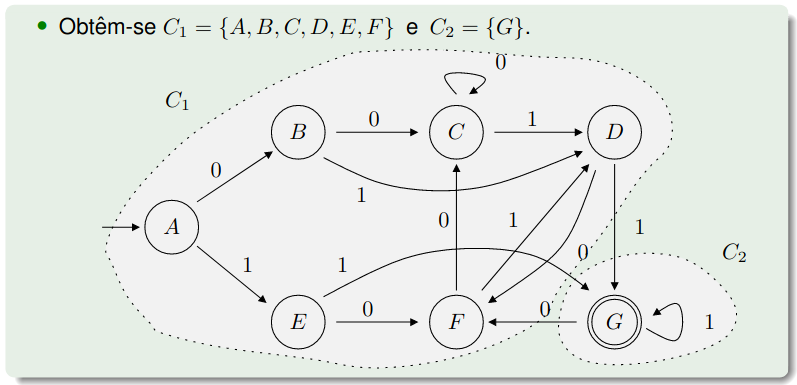
\includegraphics[scale=0.4]{43}
  \end{center}

  \item Em $C_1$, as transições em 0 são todas internas, mas em 1 podem ser internas
  ou provocar uma ida para $C_2$. Logo, não representa uma classe de equivalência e tem de ser dividido.

  \begin{center}
    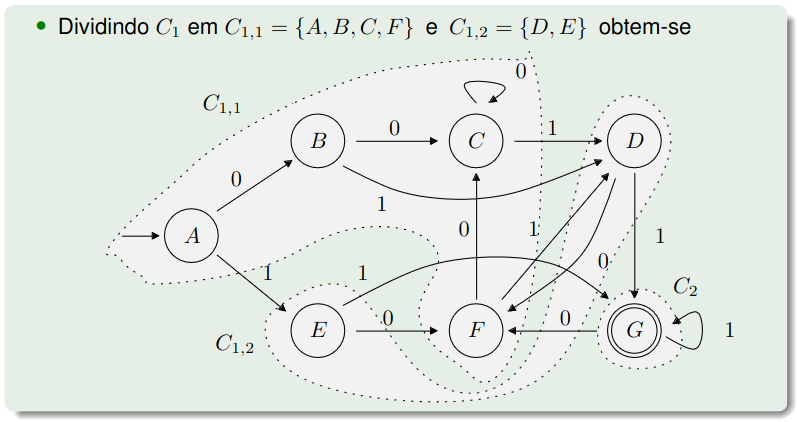
\includegraphics[scale=0.395]{44}
  \end{center}

  \pagebreak

  \item Pode verificar-se que $C_{1,1}$, $C_{1,2}$ e $C_2$ são classes de equivalência, pelo que se
  chegou à versão reduzida do autómato.

  \begin{center}
    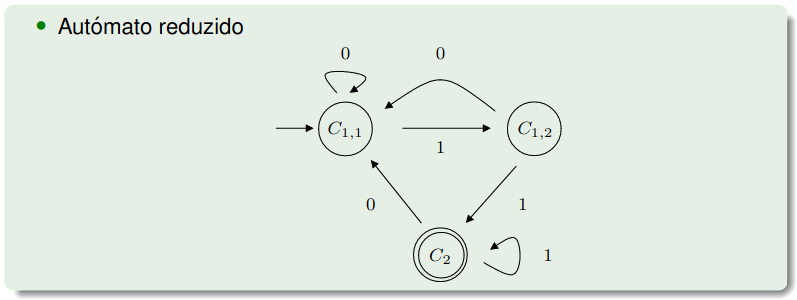
\includegraphics[scale=0.4]{45}
  \end{center}
\end{flushleft}

\subsection{Autómato finito não determinista}

\vspace{3mm}

\begin{flushleft}
  \begin{center}
    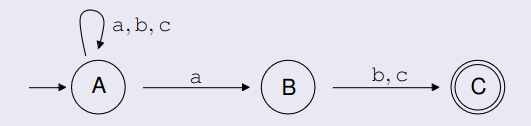
\includegraphics[scale=0.45]{46}
  \end{center}

  \item Um \textbf{autómato finito não determinista} é um autómato finito onde:
  \begin{itemize}
    \item as transições estão associadas a símbolos individuais do alfabeto \textbf{ou à palavra vazia ($\varepsilon$)};
    \item de cada estado saem \textbf{zero ou mais} transições por cada símbolo do \textbf{alfabeto ou $\varepsilon$};
    \item há um estado inicial;
    \item há 0 ou mais estados de aceitação, que determinam as palavras aceites;
    \item os caminhos que começam no estado inicial e terminam num estado de aceitação representam as palavras aceites (reconhecidas) pelo autómato;
    \item As transições múltiplas ou com $\varepsilon$ permitem alternativas de reconhecimento;
    \item As transições ausentes representam quedas num estado \textbf{morte} (estado não representado).
  \end{itemize}

  \subsubsection{AFND: caminhos alternativos}

  \begin{center}
    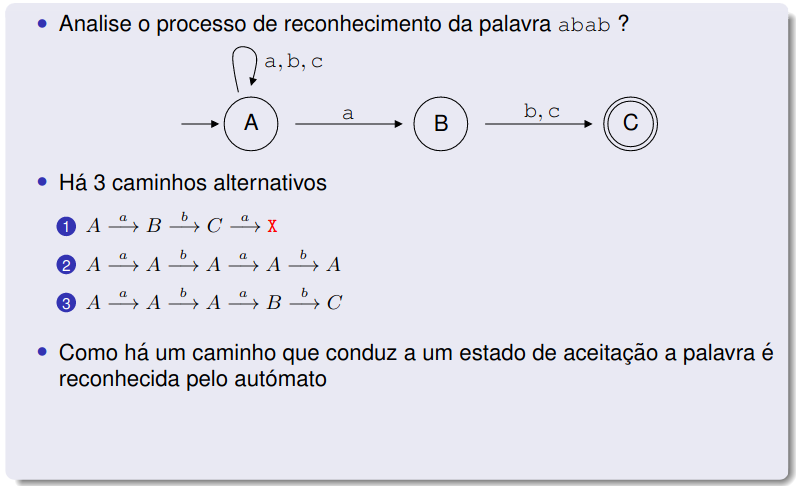
\includegraphics[scale=0.4]{47}
  \end{center}

  \begin{center}
    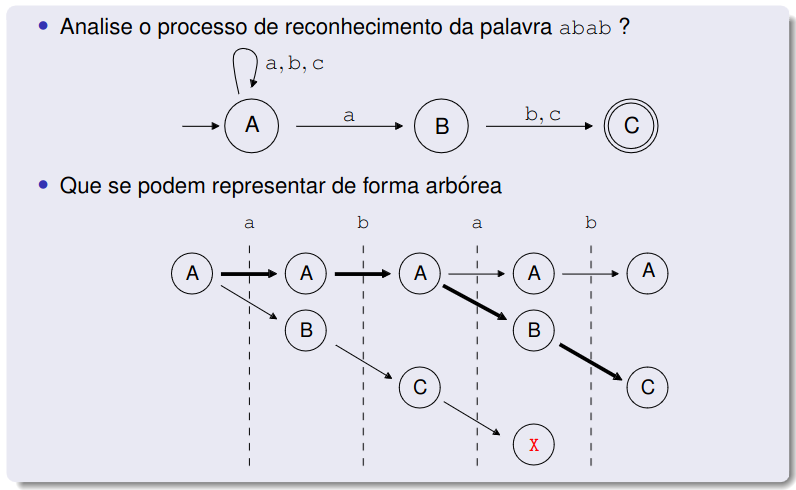
\includegraphics[scale=0.4]{48}
  \end{center}

  \pagebreak

  \subsubsection{Exemplo}

  \begin{center}
    \includegraphics[scale=0.4]{49}
  \end{center}

  Percebe-se uma grande analogia entre este autómato e a expressão regular: $(a|b|c)^* a(b|c)$

  \subsubsection{AFND com transições - $\varepsilon$}

  \begin{center}
    \includegraphics[scale=0.4]{50}
  \end{center}

  \item A palavra \textbf{101} é reconhecida pelo autómato através do caminho:
  \[A \xlongrightarrow{1} B \xlongrightarrow{0} C \xlongrightarrow{1} D\]

  \item A palavra \textbf{11} é reconhecida pelo autómato através do caminho:
  \[A \xlongrightarrow{1} B \xlongrightarrow{\varepsilon} C \xlongrightarrow{1} D\]
  \begin{center}
    porque $11$ = $1\varepsilon1$ 
  \end{center}

  \item  Este autómato reconhece as palavras terminadas em \textbf{11} ou \textbf{101}.
  \item \[L = \{w_1w_2 : w_1 \in A^* \wedge w_2 \in \{11, 101\}\}\]
\end{flushleft}

\subsubsection{Definição}

Um autómato finito não determinista (AFND) é um quíntuplo $M = (A, Q, q_0, \delta, F)$, em que:
\begin{itemize}
  \item $A$ é o alfabeto de entrada;
  \item $Q$ é um conjunto finito não vazio de estados;
  \item $q_0 \in Q$ é o estado inicial;
  \item $\delta \subseteq (Q \times A_\varepsilon \times Q)$ é a relação de transição entre estados, com $A_\varepsilon = A \cup \{\varepsilon\}$;
  \item $S \subseteq Q$ é o conjunto dos estados de aceitação.
\end{itemize}

\begin{flushleft}
  \item Apenas a definição de $\delta$ difere em relação aos AFD.
  \item Se se representa $\delta$ na forma de uma tabela, as células são preenchidas com elementos de
  $\wp(Q)$, ou seja, sub-conjuntos de Q.
\end{flushleft}

\pagebreak

\subsubsection{Exemplo}

\begin{center}
  \includegraphics[scale=0.4]{51}
\end{center}

\begin{flushleft}
  O par $(A, 1, A)$, $(A, 1, B)$ faz com que $\delta$ não seja uma função.
\end{flushleft}

\subsubsection{AFND: linguagem reconhecida}

\begin{flushleft}
  Diz-se que um AFND $M = (A,Q, q_0, \delta, F)$, \textbf{aceita} uma palavra $u \in A^*$
  se $u$ se puder escrever na forma $u = u_1u_2 \dots u_n$, com $u_i \in A_\varepsilon$ e existir uma sequência de estados
  $s_0,s_1, \dots, s_n$, satisfaça as seguintes condições:
  \begin{itemize}
    \item $s_0 = q_0$;
    \item qualquer que seja o $i = 1, \dots, n, (s_{i-1}, u_i, s_i) \in \delta$;
    \item $s_n \in F$.
  \end{itemize}
  \item Caso contrário diz-se que M \textbf{rejeita} a entrada.
  \item Note que $n$ pode ser maior que $|u|$, porque alguns $u_i$ podem ser $\varepsilon$.
  \item Usar-se-á a notação $q_i \xlongrightarrow{u} q_j$ para indicar que a palavra $u$ permite ir do estado $q_i$ ao estado $q_j$.
  \item Usando esta notação tem-se $L(M) = \{u : q_0 \xlongrightarrow{u} q_f \wedge q_f \in F\}$.
\end{flushleft}

\subsubsection{Exemplo}

\begin{center}
  \includegraphics[scale=0.4]{52}
\end{center}

\pagebreak

\subsubsection{Equivalência entre AFD e AFND}

\begin{flushleft}
  \item A classe das linguagens cobertas por um AFD é a mesma que a classe das linguagens
  cobertas por um AFND.
  \item Isto significa que:
  \begin{itemize}
    \item Se $M$ é um AFD, então $\exists_{M\rq \in AFND} : L(M\rq) = L(M)$
    \item Se $M$ é um AFND, então $\exists_{M\rq \in AFD} : L(M\rq) = L(M)$
  \end{itemize}
  \item  Como determinar um AFND equivalente a um AFD dado?
  \item Pelas definições de AFD e AFND, um AFD é um AFND. Porquê?
  \begin{itemize}
    \item $Q, q_0$ e $F$ têm a mesma definição.
    \item Nos AFD, $\delta : Q \times A \longrightarrow Q$.
    \item Nos AFND, $\delta \subset Q \times A_\varepsilon \longrightarrow Q$.
    \item Mas, se $\delta : Q \times A \longrightarrow Q$ então $\delta \subseteq Q \times A \times Q \subset Q \times A_\varepsilon \times Q$.
    \item Logo, um AFD é um AFND.
  \end{itemize}

  \subsubsection{Equivalente AFD de um AFND}

  Como determinar um AFD equivalente a um AFND dado?

  \begin{center}
    \includegraphics[scale=0.4]{53}
  \end{center}

  \begin{center}
    \includegraphics[scale=0.4]{54}
  \end{center}

  \item $\varepsilon$-closure(q) é o conjunto de estados constituído por $q$ mais todos os direta ou
  indiretamente alcançáveis a partir de $q$ apelas por transições-$\varepsilon$
  \item Note que:
  \begin{itemize}
    \item O estado inicial ($q_0\rq$) pode conter 1 ou mais elementos de $Q$;
    \item Cada elemento do conjunto de chegada ($g\rq \in F\rq$) por conter elementos de $F$ e $Q - F$.
  \end{itemize}

  \vspace{5mm}

  \textbf{Exemplo}

  \begin{center}
    \includegraphics[scale=0.4]{55}
  \end{center}

  \begin{center}
    \includegraphics[scale=0.4]{56}
  \end{center}

  \pagebreak

  \textbf{Mais um exemplo (passos nos slides)}

  \begin{center}
    \includegraphics[scale=0.4]{57}
  \end{center}
\end{flushleft}

\subsubsection{Operações sobre AFD e AFND}

\begin{flushleft}
  Os automátos finitos (AF) são fechados sobre as operações de:
  \begin{itemize}
    \item Reunião
    \item Concatenação
    \item Fecho
    \item Interseção
    \item Complementação
  \end{itemize}\vspace{5mm}

  \textbf{Reunião de AF}\break

  \begin{center}
    \textbf{Q -} Como criar um AF que represente a reunião destes dois AF?

    \includegraphics[scale=0.4]{58}
  \end{center}

  \pagebreak

  \begin{center}
    Acrescenta-se um novo estado que passa a ser o inicial, e acrescentam-se transições-$\varepsilon$
    deste novo estado para os estados iniciais originais.

    \includegraphics[scale=0.4]{59}
  \end{center}

  \textbf{Reunião de AF: definição}

  \begin{center}
    \includegraphics[scale=0.4]{60}
  \end{center}

  \textbf{Reunião de AF: exemplo}

  \begin{center}
    \includegraphics[scale=0.4]{61}
    \includegraphics[scale=0.4]{62}
  \end{center}
  \vspace{5mm}

  \textbf{Concatenação de AF}

  \begin{center}
    \textbf{Q -} Como criar um AF que represente a concatenação destes dois AF?
    \includegraphics[scale=0.4]{63}
  \end{center}

  \begin{center}
    O estado inicial passa a ser o estado inicial do AF da esquerda.

    Os estados de aceitação são apenas os estados de aceitação do AF da direita.

    Acrescentam-se transições-$\varepsilon$ dos (antigos) estados de aceitação do AF da esquerda
    para o estado inicial do AF da direita.

    \includegraphics[scale=0.4]{64}
  \end{center}

  \pagebreak

  \textbf{Concatenação de AF: definição}

  \begin{center}
    \includegraphics[scale=0.4]{65}
  \end{center}

  \textbf{Concatenação de AF: exemplo}

  \begin{center}
    \includegraphics[scale=0.4]{66}
  \end{center}
  \vspace{5mm}

  \textbf{Fecho de AF}

  \begin{center}
    \textbf{Q -} Como criar um AF que represente o fecho deste AF?
    \includegraphics[scale=0.4]{67}
  \end{center}

  \pagebreak

  \begin{center}
    Acrescenta-se um novo estado que passa a ser o inicial.

    O novo estado inicial é de aceitação.

    Acrescenta-se transições-$\varepsilon$ dos estados de aceitação do AF para o estado inicial original.

    \includegraphics[scale=0.4]{68}
  \end{center}

  \begin{center}
    Ou acrescenta-se transições-$\varepsilon$ dos estados de aceitação do AF para o novo estado inicial
    (caso em que antigos estados de aceitação podem deixar de o ser).

    Note que em geral não se pode fundir o novo estado inicial com o antigo.

    \includegraphics[scale=0.4]{69}
  \end{center}

  \textbf{Fecho de AF: definição}

  \begin{center}
    \includegraphics[scale=0.4]{70}
  \end{center}

  \pagebreak

  \textbf{Fecho de AF: exemplo}

  \begin{center}
    \includegraphics[scale=0.4]{71}
  \end{center}
  \vspace{5mm}

  \textbf{Interseção de AF}

  \begin{center}
    Como criar um AF que represente a interseção de $L_1$ e $L_2$?

    Controi-se AF para as linguagens e definir os estados que resultam do produto
    cartesiano $\{S_1, X_1\} \times \{S_2, X_2\}$. No entanto, alguns podem ser inalcançáveis.

    \begin{center}
      \includegraphics[scale=0.4]{72}
    \end{center}
  \end{center}

  \textbf{Interseção de AF: definição}

  \begin{center}
    \includegraphics[scale=0.4]{73}
  \end{center}

  \pagebreak

  \textbf{Concatenação de AF}

  \begin{center}
    Como criar um AF que represente o complemento de $L_1$?

    Considerando $L_1$ como um AFND, obtém-se um determinista equivalente e completa-se
    com os estados de aceitação.

    \begin{center}
      \includegraphics[scale=0.4]{74}
    \end{center}
  \end{center}

\end{flushleft}

\subsubsection{Equivalência entre ER e AF}

\begin{flushleft}
  \item A classe das linguagens cobertas por expressões regulares (ER) é a mesma que
  a classe das linguagens cobertas por autómatos finitos (AF).
  \item Logo:
  \begin{itemize}
    \item Se $e$ é uma ER, então $\exists_{M \in AF} : L(M) = L(e)$;
    \item Se $M$ é um AF, então $\exists_{e \in ER} : L(e) = L(M)$.
  \end{itemize}
  \item Isto indroduz duas operações:
  \begin{itemize}
    \item Como converter uma ER num AF equivalente;
    \item Como converter um AF numa AF equivalente.
  \end{itemize}
\end{flushleft}



\begin{flushleft}
  \textbf{Abordagem}

  \item Já se viu anteriormente que uma ER qualquer é:
  \begin{itemize}
    \item ou um elemento primitivo;
    \item ou uma expressão do tipo \textcolor{BrickRed}{$e_1 | e_2$}, sendo \textcolor{BrickRed}{$e_1$} e
    \textcolor{BrickRed}{$e_2$} duas expressões regulares quaisquer;
    \item ou uma expressão do tipo \textcolor{BrickRed}{$e_1  e_2$}, sendo \textcolor{BrickRed}{$e_1$} e
    \textcolor{BrickRed}{$e_2$} duas expressões regulares quaisquer;
    \item ou uma expressão do tipo \textcolor{BrickRed}{$e^*$}, sendo \textcolor{BrickRed}{e} uma expressão regular qualquer.
  \end{itemize}
  \item Já se viu anteriormente como realizar a \textbf{reunião}, \textbf{concatenação} e \textbf{fecho} de autómatos finitos.
  \item Então, se se identificar autómatos finitos equivalentes às expressões regulares primitivas,
  tem-se o problema da conversão de uma expressão regular para uma autómato finito resolvido.

  \begin{center}
    \includegraphics[scale=0.4]{75}
  \end{center}
  \item Na realidade, o autómato referente a $\varepsilon$ pode ser obtido aplicando o fecho ao autómato de $\emptyset$.
  \break

  \textbf{Algoritmo de conversão}

  \begin{itemize}
    \item Se a expressão regular é do tipo primitivo, o autómato correspondente pode ser obtido na tabela anterior;
    \item Se é do tipo $e^*$, aplica-se este mesmo algoritmo na obtenção de um autómato equivalente à expressão regular
    $e$ e, de seguida, aplica-se o fecho de autómatos;
    \item Se é do tipo $e_1e_2$, aplica-se este mesmo algoritmo na obtenção de autómatos para as expressões $e_1$ e $e_2$ e, de seguida,
    aplica-se a concatenação de autómatos;
    \item Finalmente, se é do tipo $e_1 | e_2$, aplica-se este mesmo algoritmo na obtenção de autómatos para as expressões $e_1$ e $e_2$ e, de seguida,
    aplica-se a reunião de autómatos.
  \end{itemize}

  \item Na realidade, o algoritmo corresponde a um processo de decomposição arbórea a partir da raiz seguido de um processo de construção
  arbórea a partir das folhas.
\end{flushleft}

\begin{flushleft}
  \textbf{Exemplo}

  \begin{center}
    \includegraphics[scale=0.4]{76}
  \end{center}

  \begin{center}
    \includegraphics[scale=0.4]{77}
  \end{center}
  \begin{center}
    \includegraphics[scale=0.4]{78}
  \end{center}
  \begin{center}
    \includegraphics[scale=0.4]{79}
  \end{center}
  \begin{center}
    \includegraphics[scale=0.4]{80}
  \end{center}
\end{flushleft}

\begin{flushleft}
  \subsection{Autómato finito generalizado (AFG)}

  \item Um \textbf{autómato finito generalizado (AFG)} é um quíntuplo $M = (A,Q,q_0, \delta, F)$, em que:
  \begin{itemize}
    \item $A$ é o alfabeto de entrada;
    \item $Q$ é um conjunto finito não vazio de estados;
    \item $q_0 \in Q$ é o estado inicial;
    \item $\delta \subseteq (Q \times E \times Q)$ é a relação de transição entre estados, sendo $E$ o conjunto das
    expressões regulares definidas sobre $A$;
    \item $F \subseteq Q$ é o conjunto dos estados de aceitação.
  \end{itemize}
  \item A diferença em relação ao AFD e AFND está na definição da relação $\delta$. Neste caso as etiquetas são \uline{expressões regulares}.
  \item Com base nesta definição os AFD e os AFND são autómatos finitos generalizados.
  \break

  \begin{center}
    \includegraphics[scale=0.4]{81}
  \end{center}

  \item Note que a etiqueta das transições $A \longrightarrow A$ e $B \longrightarrow B$ é $a|b|c$ (uma expressão regular) e
  não $a,b,c$ (que representa 3 transições, uma em $a$, uma em $b$ e uma em $c$).

  \begin{center}
    \includegraphics[scale=0.4]{82}
  \end{center}

  \item Note que se usou '.' e não . , porque o último é uma expressão regular que representa
  qualquer letra do alfabeto.

  \subsubsection{Conversão de um AFG numa ER}

  \begin{center}
    \includegraphics[scale=0.4]{83}
  \end{center}

  \item Note que:
  \begin{itemize}
    \item O estado $A$ não é de aceitação e não tem transições a chegar;
    \item O estado $B$ é de aceitação e não tem transições a sair.
  \end{itemize}
  \item Se se reduzir um AFG à forma anterior, $e$ é uma expressão regular equivalente ao autómato
  \item O processo de conversão resume-se assim à conversão de AFG à forma reduzida.

  \textbf{Algoritmo de conversão}

  \begin{enumerate}
    \item transformação de um AFG noutro cujo estado inicial \textbf{não tenha transições a chegar}
    \begin{itemize}
      \item Se necessário, acrescenta-se um novo estado inicial com uma transição em $\varepsilon$ para o antigo
    \end{itemize}
    \item transformação de um AFG noutro com \textbf{um único estado de aceitação, sem transições de saída}
    \begin{itemize}
      \item Se necessário, acrescenta-se um novo estado, que passa a ser o único de aceitação, que recebe
      transições em $\varepsilon$ dos anteriores estados de aceitação, que deixam de o ser
    \end{itemize}
    \item Eliminação dos estados intermédios
    \begin{itemize}
      \item Os estados são eliminados um a um, em processos de transformação que mantêm a equivalência
    \end{itemize}
  \end{enumerate}
\end{flushleft}

\pagebreak

\begin{flushleft}
  \textbf{Algoritmo de eliminação de um estado}

  \begin{center}
    \includegraphics[scale=0.4]{84}
  \end{center}
  \begin{center}
    \includegraphics[scale=0.4]{85}
  \end{center}
\end{flushleft}

\subsection{Equivalência entre GR e AF}

\begin{flushleft}
  \item  A classe das linguagens cobertas por gramáticas regulares (ER) é a mesma que a classe das linguagens cobertas por autómatos finitos (AF).
  \item Logo:
  \begin{itemize}
    \item Se $G$ é uma ER, então $\exists_{M \in AF} : L(M) = L(G)$
    \item Se $M$ é uma ER, então $\exists_{G \in ER} : L(G) = L(M)$
  \end{itemize}
  \item Isto introduz duas operações:
  \begin{itemize}
    \item Como converter um AF numa GR equivalente
    \item Como converter uma GR num AF equivalente
  \end{itemize}

  \pagebreak

  \subsubsection{Conversão de um AF numa GR}

  \begin{center}
    \includegraphics[scale=0.4]{86}
  \end{center}

  \textbf{Exemplo}
  \begin{center}
    \includegraphics[scale=0.4]{87}
  \end{center}
\end{flushleft}

\pagebreak

\subsubsection{Conversão de uma GR num AFG}

\begin{center}
  \includegraphics[scale=0.4]{88}
\end{center}

\textbf{Exemplo}

\begin{center}
  \includegraphics[scale=0.4]{89}
\end{center}


\end{document}